%!TEX root = documentation.tex

\chapter{Master}

\section{About the Master} % (fold)
\label{sec:about_the_master}

The master is written Java and uses the jamod Library\footnote{\url{http://jamod.sourceforge.net/}} for the communication with the sensors over the modbus protocoll. The view is created with the SWT Library\footnote{\url{http://www.eclipse.org/swt/}}. 
It's seperated in several parts:
\begin{itemize}
	\item View (see \ref{sec:view})
	\item Configuration (see \ref{sec:configuration})
	\item Stations  (see \ref{sec:stations})
	\item History (see \ref{sec:history})
\end{itemize}

It's needed to create a configuration file before collection process of the measurement values could be started. A sensor must be added to the master befor it can be used. Each sensor has a individual name and ip address and it's refered as a station. In the configuration phase it's nesseary to specify the kind of data that the stations collect. The data that is transfered from the station to the master is called Input Parameter. To configure the sensor it's possible to define configuration Parameters. These values are transfered from the master to the sensor. To map the parameters to the memory in the station they must be bound to addresses. This happens individually for each station. So it's possible to collect different data from different stations. It's also possible to configure the kind of plots that are generated (see \ref{sub:plots}).

After the configuration of the stations the collection process could be started. Each station is polled in its own thread. One collector thread collects the data from all stations, generates a text file with the information about the current values from the stations and draws the plots. The time between the polling of the stations and between generation of the output files can also be configured. As soon the current day changes the values from the last day are aggregated to a history value. This daily history is kept for one year. The values from the station are kept for two days so it's possible to plot hourly data. 

% section about_the_master (end)

\section{View} % (fold)
\label{sec:view}

The view is created with the help of SWT. SWT uses the os drawing apis to draw the widgets. So the look and feel of the application is very good integrated in the os it runs in. 

\subsection{Screenshots} % (fold)
\label{sub:screenshots}

\begin{figure}[ht]
    \centering
    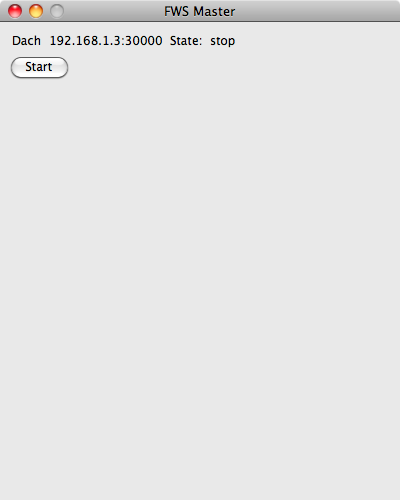
\includegraphics[width=0.6\linewidth]{master/mainview.png}
    \caption{Quick overview about the stations and their status}
    \label{fig:main}
\end{figure}

\begin{figure}[ht]
    \centering
    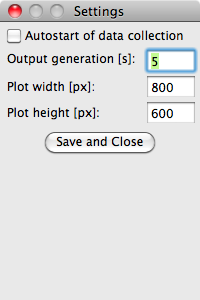
\includegraphics[width=0.4\linewidth]{master/settings.png}
    \caption{Configuration of the basic settings}
    \label{fig:settings}
\end{figure}

\begin{figure}[ht]
    \centering
    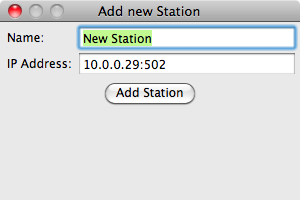
\includegraphics[width=0.6\linewidth]{master/add.png}
    \caption{Adds a new station to the master}
    \label{fig:add}
\end{figure}

% TODO bilder mit sinnvoller config einfügen
%\begin{figure}[ht]
%    \centering
%    \includegraphics[width=0.8\linewidth]{master/parameter.png}
%    \caption{Adding/editing of the parameters}
%    \label{fig:parameter}
%\end{figure}

%\begin{figure}[ht]
%    \centering
%    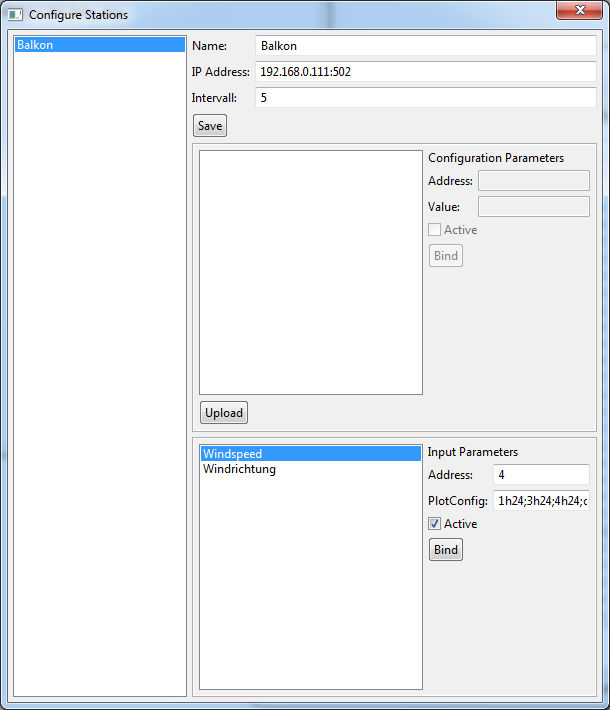
\includegraphics[width=0.8\linewidth]{master/stations.png}
%    \caption{Editing station specific settings. The parameters bindings are also set here}
%    \label{fig:stations}
%\end{figure}
%
%\begin{figure}[ht]
%    \centering
%    \includegraphics[width=0.8\linewidth]{master/data.png}
%    \caption{Shows the currently collected and saved data}
%    \label{fig:data}
%\end{figure}
% subsection screenshots (end)

\section{Configuration} % (fold)
\label{sec:configuration} 
%TODO enabled wenn vorhanden
The nessesary views for the configuration are \ref{fig:add}, \ref{fig:settings}, %\ref{fig:parameters} and \ref{fig:stations}.

The result of the configuration phase is an xml file with all settings in it. See example in Listing \ref{code:settings}

{\C \lstinputlisting[language=xml,breaklines=true,caption={Sample settings file},label=code:settings,frame=tlRB]{master/settings.xml} }

\subsection{Parameters} % (fold)
\label{sub:parameters}
There are two types of parameters. Input Parameters and Configuraton Parameters. Each parameters has a unique name and a boolean value if it's enabled. The name is the identifyer of the parameters so it has to be unique. Beside of these common attributes the configuration and input parameters have further attributes.

\subsubsection{Input Parameter} % (fold)
\label{ssub:input_parameter}
Additional attributes of an input parameter:
\begin{itemize}
	\item Unit
	\item Format
	\item History Funtion
\end{itemize}

\paragraph{Unit} % (fold)
\label{par:unit}
The Unit is just used for the description in the generated files. Availible units are:
\begin{itemize}
	\item speed $\frac{m}{s}$
	\item speed $\frac{km}{h}$
	\item frequenzy $Hz$
	\item direction
	\item temperatur $^\circ C$
\end{itemize}

% paragraph unit (end)

\paragraph{Format} % (fold)
\label{par:format}
The transfered value from the station is a 16 bit integer value. To be able to display floating point numbers it's possible to set the output format to the desired form. Example: The temperatur equals $23.3 ^\circ C$. The station measures the temperatur and converts it to $233$ to have an integer value. On the master the output format is set to the format with one digit before the decimal point. When such an input parameter is used it's converted back to $23.3$.

\paragraph{History Function} % (fold)
There are three different history functions availible. For more details about these functions and how they are used please read \ref{sec:history}.
\label{par:history_function}
\begin{itemize}
    \item average
    \item minimum
    \item maximum
\end{itemize}
% paragraph history_function (end)
% paragraph format (end)
% subsubsection input_parameter (end)

\subsubsection{Configuration Parameter} % (fold)
\label{ssub:configuration_parameter}
Additional attributes of a configuration parameter:
\begin{itemize}
    \item value
\end{itemize}

\paragraph{Value} % (fold)
\label{par:value}
A configuration parameter is a value that is transfered from the master to the slave. The value that is transfered is saved in the attribute value. This value must be an 16 Bit integer value.
% paragraph value (end)
% subsubsection configuration_parameter (end)

% subsection parameters (end)

\subsection{Plots} % (fold)
\label{sub:plots}
The plots are generated with the help of the jFreeChart Library \footnote{\url{http://www.jfree.org/jfreechart/}}.
The plots can be configured for every binding. Each binding can have several plots asigned. It's also possible to plot more than one data into one plot. The plots are configured with a string. The simplest configuration looks like {C h24;} With that configuration one plot is generated and the data for this plot are the values from the last 24 hours. The plots are generated in the output directory that can be set from the user.

It's possible to use differnt data ranges for the plots. To allow the use to choose one range are three differnt time bases availible:
\begin{itemize}
	\item c - current
	\item h - hours
	\item d - days
\end{itemize}

\paragraph{Current} % (fold)
\label{par:current}
Use the last values for the plot. Currently this is only implemented for the wind direction. Results in an plot like Figure \ref{fig:current}.
\begin{figure}[ht]
    \centering
    
\includegraphics[width=0.9\linewidth]{master/plot_examplec.png}
    \caption{Current Wind direction plot}
    \label{fig:current}
\end{figure}
% paragraph current (end)

\paragraph{Hours} % (fold)
\label{par:hours}
Use the last values of the last hours for the plot. The ammount of the hours is specified in the plot configuration. It's the number after the timebase. Example of an 24 hour plot see Figure \ref{fig:hours}.
\begin{figure}[ht]
    \centering
    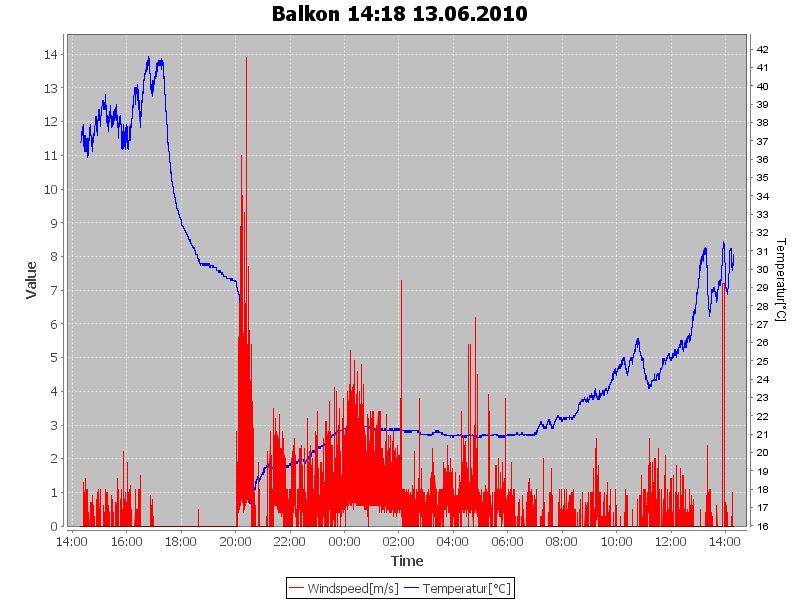
\includegraphics[width=0.9\linewidth]{master/plot_exampleh.png}
    \caption{last 24 hours of two seperat parameters in one plot}
    \label{fig:hours}
\end{figure}
% paragraph hours (end)

\paragraph{Days} % (fold)
\label{par:days}
Same plot as with the hours timebase but the values from the last days are used. For more details about the history see chapter \ref{sec:history}.
% paragraph days (end)

\subsubsection{Configuration Syntax} % (fold)
\label{ssub:configuration_syntax}
Each plot is specified by three different parts: [Number]CharacterNumber;

\paragraph{First Number: ID} % (fold)
\label{par:first_number_id}
This number is optional and controlls if more than one input parameter is drawn in one plot. All configured plots with the same number are drawn in the same plot.
% paragraph first_number_id (end)
\paragraph{Character: Timebase} % (fold)
\label{par:character}
Defines the timebase. Explained in paragraphes above.
% paragraph character (end) 
\paragraph{Second Number: Ammount of data} % (fold)
\label{par:number}
The second number defines how much data will be in the plot. d4; will plot the last four days.
% paragraph number (end)
\paragraph{End of Configuration} % (fold)
\label{par:end_of_configuration}
Each configuration must end with an {\C `;'}.
% paragraph end_of_configuration (end)

\paragraph{Example} % (fold)
\label{par:example}
For the configuration string {\C h24;1h24;d30;c1;d365;} following plots are generated:
\begin{itemize}
	\item Last 24 hours
	\item Last 24 hours with other data with ID 1 
	\item Last 30 days
	\item Current value
	\item Last 365 days
\end{itemize}

% paragraph example (end)
% subsubsection configuration_syntax (end)

\subsubsection{Detailed Information about the plots} % (fold)
\label{ssub:detailed_information_about_the_plots}
If two differnt data sets should be ploted in one plot there two axis with own scale generated. When more that three data sets should be drawn in one plot they share one axis. So it's advisable to generate more plots with two datasets each in it to kepp the plots tidy.

The direction parameters values are not connected with a line. Otherwise the plot would be unreadable if the wind directions changes a lot.

The direction parameter values are mapped to a description of the direction. So $0^\circ$ result in N(orth) see figure \ref{fig:dir}
\begin{figure}[ht]
    \centering
    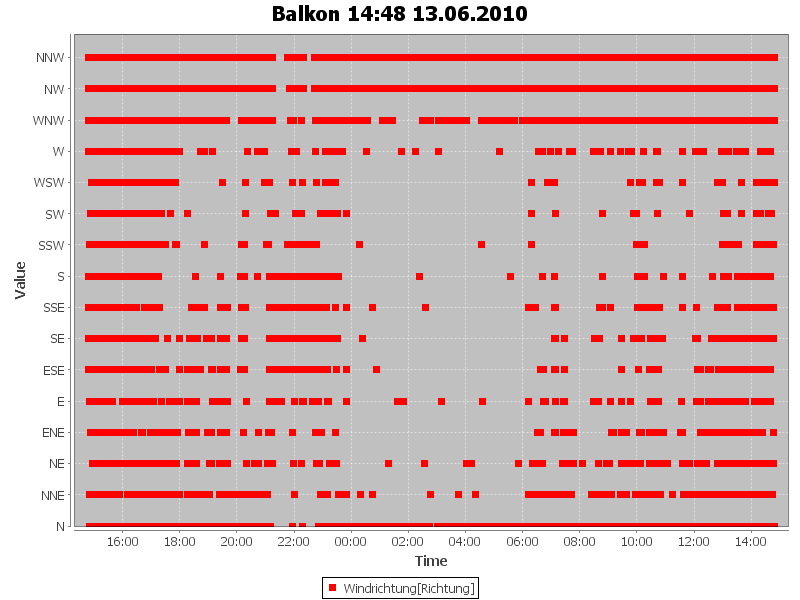
\includegraphics[width=0.9\linewidth]{master/plot_dir.png}
    \caption{Axis description of direction parameter}
    \label{fig:dir}
\end{figure}
% subsubsection detailed_information_about_the_plots (end)
% subsection plots (end)
% section configuration (end)

\section{Stations} % (fold)
\label{sec:stations}

% section stations (end)

\section{History} % (fold)
\label{sec:history}

% section history (end)